\section{Validation}

%This part of the thesis the thesis deals with the numerical validation of the immersed
%boundary methods
%In the first part of the chapter an introduction to different test cases
%will be given. Three different test problems were chosen.
%The flow between to planes, also known as Planar Poiseuille flow, the flow in a Pipe, referred to as Hagen-Poiseuille flow and the flow
%between two rotating cylinders, know as the Taylor-Couette system.
%In the second part of the chapter the result for the different test cases will be presented and discussed.
%In the first part of the chapter an introduction to different test cases
%will be given.
This section presents the numerical validation of the immersed boundary methods.
The objective of the validation is to determine the numerical accuracy and
the numerical stability for each method.
Furthermore, it is important to test if conservation laws, in particular the conservation of mass,
are fulfilled.
For the validation three different test problems were chosen.
The flow between two parallel planes, also known as planar Poiseuille flow, the flow in a Pipe, referred to as Hagen-Poiseuille flow and the flow
between two rotating cylinders, known as the Taylor-Couette system.

\paragraph{Conventions}\mbox{}\\

In this section the following abbreviations will be used

\begin{multicols}{2}
\begin{description}
    \item[VP]{Volume-Penalization Method}
    \item[DF]{Direct Forcing Method}
    \item[IP]{Interpolation Method}
    \item[VF]{Volume-Fraction Method}
    \item[FD2]{Finite Difference Schemes of second order}
    \item[FD4]{Finite Difference Schemes of fourth order}
\end{description}
\end{multicols}

For example, DF-VF FD2 method, refers to the Direct-Forcing method, extended with the Volume-Fraction
method and the use of 2nd order finite difference schemes.

\paragraph{Grid Convergence Studys}\mbox{}\\

For the validation multiple grid convergence studys were performed.
The concept of a grid convergence study is to vary the grid resolution of the numerical domain and
calculate the error of the simulation with respect to an assumed theoretical solution.
The relative error $\epsilon$ is computed by the $l_2$-norm by (see \citep{QUELLE})

\begin{align}
    \epsilon = \frac{\int \dif V \left(\Phi^{\text{th}} - \Phi^{\text{num}}\right)^2}{\int \dif V \left( \Phi^{\text{th}} \right)^2}
     = \frac{\sum_{i,j,k}^{N_x, N_y, N_z}
      \left(\Phi^{\text{th}}_{i,j,k}  - \Phi^{\text{num}}_{i, j, k}  \right)^2}
     {\sum_{i,j,k}^{N_x, N_y, N_z} \left( \Phi^{\text{th}}_{i,j,k} \right)^2}
 \end{align}

where $\Phi^{\text{th}}$ corresponds to the theoretical and $\Phi^{\text{num}}$ to the numerical solution of any field variable $\Phi$.
The numerical error is often given by a power law of the form $\epsilon = N^\lambda$, i.e for a finite difference scheme of 2nd order
this is the truncation error given by the remaining terms  of the taylor expansion.
For an evaluation of the error convergence the results of the grid convergence study are, if possible, linear fitted in the log-log space, to obtain the
convergence rate $\lambda$.

%In general it is necessary to obtain a good evaluation of the numerical truncation error,
% the numerical stability over longer periods of time
%and Grid convergence studys against theoretical and high-resolution numerical solutions
%will be performed and compared for the different IBMs.
%In order to ensure a correct numerical behavior of the introduced methods, a
%Multiple examples from simple to more complex test cases are introduced in this section.
\clearpage

\subsection{Laminar Poiseuille Flow}
\label{vali:sec_lpflow_setup}

\begin{figure}[!bp]
  \begin{minipage}[c]{0.6\textwidth}
      \centering
        \resizebox{0.9 \textwidth}{!}{
       \import{gfx/immersed_boundary/poiseuille_flow//}{setup.pdf_tex}
      }
  \end{minipage}
  \begin{minipage}[c]{0.3\textwidth}
      \caption{Flow in a channel of height $\Delta h = h_2 - h_1$, with periodic boundaries in $x$ and $y$ direction and
       a predefined pressure gradient $\nabla p$.
      \label{validation:setup_pf}
      }
  \end{minipage}
\end{figure}

The numerical setup of this test case is presented in Fig. \ref{validation:setup_pf}.
It consist of two infinite extending  planes at $z=h_1$ and $z=h_2$, which are oriented
parallel to the xy-plane, at a distance $\Delta h = h_2 - h_1$.
A infinite long channel is numerically realized by using periodic boundaries in x- and y-direction.
For the walls immersed boundaries, or in case of the default algorithm No-Slip boundaries, are used.
The fluid flow in the channel is a result from a predefined constant pressure gradient $\nicefrac{\partial p}{\partial x}$
in the fluid domain.
In the implementation this pressure gradient is added into the Navier-Stokes equation as an additional forcing term.
For the steady state the flow is independent of the $x$ and $y$ coordinate.
The equations of motion, here in the non-dimensional form, are according to \citep{Kundu2012} given by

\begin{align}
    \label{vali:pflow_navstok}
    \frac{\partial v_x}{\partial t} &= - \frac{\partial p}{\partial x}
     + \frac{1}{Re} \frac{\partial^2 v_x}{\partial z^2} = 0,
\end{align}

where $Re = \nicefrac{V_{m}\Delta h}{\nu}$, with the non-dimensionalization defined as

\begin{align}
    \text{Length:}\qquad &  \vec{r} = \frac{\vec{r^*}}{\Delta h}  &
    \qquad \text{Velocity:}\qquad& \vec{v} =  \frac{\vec{v^*}}{V_{\text{M}}}\\
    \text{Time:}  \qquad & t = \frac{t^* \cdot V_\text{M}}{\Delta h}&
    \qquad  \text{Pressure:}\qquad & p = \frac{\nabla p^*}{\rho V_\text{M}^2}
\end{align}
%For this system the non-dimenzionalization is given by the scales
%    $r^* = \nicefrac{r}{\Delta h}$, $v^*=\nicefrac{V_(\text{m})}{\Delta h}$,
%    $t^* = \nicefrac{V_{\text{m}}}{\Delta h}$ and $p^* = p \rho V_{\text{max}}^2$.

where $V_\text{M}$ is defined by the maximal velocity in the channel $\max(v_x(z))$.
By the integration of Eq. \ref{vali:pflow_navstok} it follows that
\begin{align}
v_x &= \frac{1}{2}\frac{\partial p}{\partial x}\Rey z^2 + zc_1 + c_2.
\end{align}

The integration constants are obtained by setting $v_x(h_1) = v_x(h_2) = 0$:
\begin{align}
c_1 = A\frac{h_1^2 -h_2^2}{h_2 - h_1} = -A(h_1+h_2)\qquad ,& \qquad
c_2 = A(h_1(h_1 + h_2) - h_1^2) = Ah_1h_2,
\end{align}

with the definition $A:=\frac{1}{2}\frac{\partial p}{\partial x} Re$.
The velocity is then given by the quadratic function
\begin{align}
\label{vali:pflow_theosol}
v_x &= A(z^2 - z(h_1 + h_2) + h_1h_2)
\end{align}

The maximum velocity and position are given by
\begin{align}
z_{\text{M}} &= \frac{h_1+h_2}{2} \wedge v_{\text{M}} = A\left(h_1h_2 - \frac{(h_1 + h_2)^2}{4}\right)
\end{align}

Due to the non-dimensionalization it is necessary that $V_{\text{M}} \overset{!}{=}  1$.
It follows that

\begin{align}
    \label{vali:pflow_pcondi}
\frac{\partial p}{\partial x} &= \frac{2}{Re}\frac{1}{\left(h_1h_2 - \frac{(h_1+h_2)^2}{4} \right)}
\end{align}

has to be fullfilled as a necessary condition for the pressure gradient.

\subsection{Simulations}

The Poiseuille flow is used in particular as a first validation test case
for the VP, DF method  and the basic implementation.

\subsubsection{Test of the Basic Setup}

The purpose of the first simulation is to test  the basic
implementation of the algorithm which does not use immersed boundaries.
For the Poiseuille flow this is still possible since the geometry is non-curved
and parallel to the cartesian grid. The heights for this setup are set to $h_1=0$ and $h_2=1$.
A grid convergence test was performed with the main simulation parameters given by
\footnote{For reasons of clarity only the important simulation parameters, depending on the setup and the performed simulation,  will be presented in this thesis.}
\footnote{The size in $l_x/l_y$ direction is set to the smallest possible value which is 8 grid points due to the GPU algorithm which uses a blocksize of 8x8.}

\begin{center}
\vspace*{0.7ex}
\begin{tabular}{c|c|c|c|c|c|c }
 $ N_z  $                   & $\Delta t$ & $\Delta z$            & $\Rey$  & $c^2$   & $l_z, l_x/l_y$ & $T_{end}$\\
\hline
 $[8, 256], \Delta N = 8 $& $10^{-4}$ & $\nicefrac{1}{N - 1}$ & 500     & $500$   &  1, 8$\Delta z$ &  10\\
\end{tabular}
\vspace*{0.7ex}
\end{center}

The simulation was performed for FD2 and FD4 methods.

\subsubsection{Test of the Volume-Penalization Method}

%With the given theoretical solution, the next objective is the comparison
%to the default implementation, the volume penalization method and the direct forcing method.
%Since we have a flow parallel to the grid  it does not make sence to compare it to the interpolation methods
%For the comparision with a theoretical solution it is necessary to ensure that
% the surface grid points match with the total height $h$ of the channel.

For the immersed boundary methods the upper and lower boundaries of the channel are realized by the masking function
\begin{align}
H(z) = \begin{cases}
                    0, & \text{for \  }  h_1 \leq z \leq h_2 \\
                    1, & \text{else}.
             \end{cases}.
\end{align}

For the VP-method an additional forcing term for Eq. \ref{vali:pflow_navstok} of the form

\begin{align}
    \vec{f} = -\frac{H}{J}\vec{v}
\end{align}

has to be introduced (see Sec. \ref{chap:ibm_volpen}),
where the non-dimensionalized damping coefficient is given by $J = \nicefrac{V_{m}}{\eta}$.
A first test is an investigation of the error of the velocity profile, with a variation of the Reynolds-number and the damping coefficient $J$.
To ensure that the channel width is equal to $\Delta h = 1$, the total height of the simulation domain was set to $l_z\approx2.01587$,
with $h_1=0.5$ and $h_2=1.5$.
This ensures that the grid points overlap exactly with the masking function at $h_1$ and $h_2$.
A simulation series was performed for the VP-FD2 method with the simulation parameters

\begin{center}
\vspace*{0.7ex}
\begin{tabular}{c|c|c|c|c|c|c|c|c }
 $ \Rey  $                      & $J$ & $N_z$ &  $\Delta t$ & $\Delta z$            & $c^2$   & $l_z, l_x/l_y$ & $T_{end}$\\
\hline
 $[100, 500], \Delta \Rey = 25 $& $[10^{-5}, 5\cdot10^{-1}]  $ & 64 &  $10^{-4}$ & $\nicefrac{1}{N - 1}$   & $500$   & $\approx{2.015871}, 8\Delta z$ & 10\\
\end{tabular}
\vspace*{0.7ex}
\end{center}

The stepping of $J$ was varied such that each order of magnitude is covered by two values, i.e. $10^{-1}$ and $5\cdot10^{-1}$.
A value of $J=10^{-5}$ corresponds to a relative strong damping force in comparison to a weak damping at a value of $J=10^{-1}$.
As a second test a grid convergence study was carried out with a constant Reynolds number,
where the resolution was varied between $N_z\in [8, 280]$ with $\Delta N_z = 8$. VP-FD2 and VP-FD4 methods were tested with the parameters

\begin{center}
\vspace*{0.7ex}
\begin{tabular}{c|c|c|c|c|c|c|c }
 $ N_z  $                      & $J$ &  $\Delta t$ & $\Delta z$            & $\Rey$  & $c^2$   & $l_z, l_x/l_y$ & $T_{end}$\\
\hline
 $[8, 280], \Delta N_z = 4 $& $[10^{-4}, 5\cdot10^{-2}]  $ &  $10^{-4}$ & $\nicefrac{1}{N - 1}$ & 500     & $500$   & $\approx{2.015871}, 8\Delta z$  & 10\\
\end{tabular}
\vspace*{0.7ex}
\end{center}

\subsubsection{Test of the Direct-Forcing Method}

Since the DF method does not depend on a damping coefficient (see Sec. \ref{chap:ibm_dirforce}),
it is sufficient enough to carry out a grid convergence study.  The simulation parameters are given by

\begin{center}
\vspace*{0.5ex}
\begin{tabular}{c|c|c|c|c|c|c }
 $ N_z  $                       &  $\Delta t$ & $\Delta z$            & $\Rey$  & $c^2$   & $l_z, l_x/l_y$ & $T_{end}$\\
\hline
 $[8, 280], \Delta N_z = 4 $ &  $10^{-4}$ & $\nicefrac{1}{N - 1}$ & 500     & $500$   & $\approx{2.015871}, 8\Delta z$  & 10\\
\end{tabular}
\vspace*{0.5ex}
\end{center}

The simulations were performed for FD2 and FD4 methods.

\clearpage

\subsection{Results}
\subsubsection{Test of the Basic Setup}

The results of the grid convergence study are shown in Fig. \ref{fig:ema1}.
The double logarithmic axis shows the dependency of the computed relative $l_2$-error norm
with respect to the grid resolution.

On this scale, the FD4 has a linear decreasing error.
For the smallest resolution $N=8$ the error is of order $10^{-3}$,
in contrast to the highest resolution $N=256$ with an error of order $10^{-6}$.
A convergence rate of the error  was computed  according to $\lambda\approx -2.26$.
Hence, it can be said that the accuracy of the method is above 2nd order for this test case,
which is is in contradiction with the theory assuming a 4th order.
The error of the 2nd order finite difference scheme is of the order $10^{-8}$.
The value is approximately constant and does not depend on the grid resolution.

\begin{figure}[!bp]
    \centering
    \includegraphics{gfx/immersed_boundary/poiseuille_flow/1_default/relative_l2error.pdf}
    \caption{Relative $l_2$-error for FD2 and FD4 methods with the basic algorithm without the use of an immersed boundary.\label{fig:ema1}}
\end{figure}


\subsubsection{Test of the Volume Penalization Method}

The first simulation was  a parameter study with variable Reynolds number and damping rate.
A first impression of the influence of the damping rate $J$ is given by the velocity profiles of the numerical solution.
This is exemplarily shown in Fig. \ref{fig:vp_flow}, for varying $J$ and $Re=500$ .
It can be noted that with an decrease of $J$, the numerical solution converges against the theoretical one.
Furthermore it can be seen that the quadratic part of the velocity profile,
inside of the fluid domain ($0.5\leq z \leq 1.5$), is independent of the damping constant $J$.
Merely a slight offset at the boundaries creates a constant shift of the velocity profile.
In the masked area of the volume a decrease in velocity is visible which could  eventually be described by an
exponential law.

\begin{figure}[!t]
  \centering
  \includegraphics{gfx/immersed_boundary/poiseuille_flow/2_vp/vp_profile.pdf}  \caption{\label{fig:vp_flow}
    Velocity profile of the numerical solution with variable $J$ and $\Rey = 500$.}
\end{figure}

For an error estimation, the relative $l_2$-error was computed, the results are shown in Fig. \ref{fig:vp_error}.
On the left side of the plot the relative error is plotted against the damping rate and the reynolds number is
varied over a color scale. On the right side both variables ($J$ and $\Rey$) are switched.

\begin{figure}[!b]
  \centering
  \includegraphics{gfx/immersed_boundary/poiseuille_flow/2_vp/vp_error.pdf}  \caption{\label{fig:vp_error}
    Relative $l_2$-error for variable damping rate $\nu$ and Reynolds number $Re$.}
  \centering
  \includegraphics{gfx/immersed_boundary/poiseuille_flow/2_vp/vp_convergence.pdf}
  \caption{\label{fig:vp_conv}
      Relative $l_2$ error for variable damping rate $J$, for VP-FD2 (blue) and VP-FD4 (red) methods.}
\end{figure}


A decrease in the damping rate $J$ results in an decrease of the error about four orders, from $10^{-1}$ to $10^{-5}$.
With a change of the Reynolds number from $500$ to $100$ the error decreases about one order.
It can be noticed that with an decrease of $\Rey$ or $J$ the error decreases linear in the log-log space.
For a small damping ($J>10^{-3}$) a breakdown of the linear relation can be observed.
This is an error resulting from the numerical setup.
The damping in the masking area is so weak that the flow reaches the  boundaries of the numerical domain.
This is not the case for $J<1e-3$ since the velocity profile is zero before it reaches the boundaries.
A linear fit in the log-log space gives a  decay rate of about $1.106$ for  $J$ and about $-1.223$ for $\Rey$.

The second part of the test was a grid convergence study with a constant Reynolds number, variable $J$ and grid resolution $N$.
The results are shown in Fig. \ref{fig:ema1}.
It can be noticed that a decrease in $J$ creates a shift in the error profile to overall smaller values.
However it is also noticable that the error of the FD2 method increases together with the resolution.

Even less understandable is the error function for the FD4 method.
With increasing resolution  a decrease into a minimum, followed by an increase can be observed.
The position of minimum is shifted to the right with an decrease of $J$.
For a constant $J>10^{-4}$ it is visible that the error for both methods converges against a
constant error  with an increase in the resolution.

\clearpage

\subsubsection{Test of the Direct Forcing Method}

The results of this grid convergence study for the DF method
are similar to the results of the basic implementation, except the DF-FD4 method has a larger error.
A plot of the relative $l_2$-error can be found in the Appendix in Fig.\ref{fig:vali_pflow_3gc}.
The FD4 method has a linear decreasing error in the log-log space.
For the smallest resolution $N=8$ the error is of order $10^{-2}$,
in contrast to the highest resolution $N=256$, with an error of order $10^{-4}$
The convergence rate is about $\lambda\approx1.267$.
Hence, it can be said that the accuracy of the method is above first order for this test case.
The error of the second order finite difference scheme is of the order $10^{-8}$.
The value is approximately constant and not depend of the grid resolution.

\subsection{Discussion}
\subsubsection{Test of the Basic Setup}

The constant error of the FD2 can be explained by the lack of complexity of the test case.
As the theoretical solution, given by Eq. \ref{vali:pflow_navstok} is a polynom of 2nd order,
no higher order terms will occur in the numerical solution.
Hence, the FD2 method is capable of a perfect approximation, independent of the
grid resolution. The remaining error terms, wich are of the order $10e^{-8}$,
occur due to the round-off error of the single precision floating-point format.

The convergence of the fourth order scheme, which is above 2nd order
reveals that an error exists in the basic implementation of the No-Slip boundaries.
An explanation can be given with a comparison to the theoretical solution.
The 2nd derivative is given by

\begin{align}
    \pdn[^2 v_x]{x^2} = \frac{1}{\Rey}\pdn[p]{x} := C\in\mathbb{R}
\end{align}

The basic algorithm uses a mirroring method on the boundaries of the fluid domain (see Sec. \ref{XXX}), for the No-Slip boundaries.
Let $C_b$ be the derivative in the immersed boundary, it follows that $C_b = - C$, as a result of the mirroring.
Therefore a discontinuity of the 2nd derivative is created at the boundaries.
When using the 2nd order method the 3-Point stencil of the FD2 method evaluates to the correct value.
The 5-Point stencil of the FD4 method evaluates to a false value, since it uses one point behind the boundary.
As a result the discontinuity creates an error in this approximation.

\clearpage

\subsubsection{Test of the Volume Penalization Method}

The offset on the boundaries arises since the VP method cannot fullfill the exact boundarie conditions.
For the steady state a force equillibrium at the boundaries is given by the pressure gradient, the laplace operator and the damping force.

\begin{align}
\label{valid:steady_state_pflow}
 \frac{H}{J} v_x &=  \frac{1}{\Rey}\frac{\partial^2 v_x}{\partial z^2} -\pdn[p]{x}
\end{align}

The result is a constant offset $v_x(h_1) = v_x(h_2) =: C\in\mathbb{R}$.
The simultaneous decrease of the $l_2$-error with $J$ is as expected, since a stronger damping force $\propto \nicefrac{1}{J}$ creates a smaller
error at the boundaries.
However it is counterintuitive that the $l_2$-error decreases with an increase of the Reynolds number.
An explanation for this is, that the viscous force and the pressure gradient are proportional to $\nicefrac{1}{\Rey}$
(see Eq. \ref{vali:pflow_pcondi}).
With an increase of the Reynolds number the left side of Eq. \ref{valid:steady_state_pflow} becomes smaller.
The damping force becomes larger in comparison and the  offset $C=v_x(h_1)=v_x(h_2)$ decreases.

\begin{figure}[!bp]%
    \centering
    \subfloat[Velocity profile at the immersed boundary for the VP-FD2 and the VP-FD4 method]{{
    \label{fig:example_a}%
      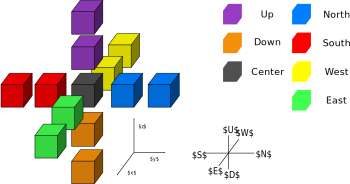
\includegraphics{gfx/immersed_boundary/poiseuille_flow/discussion/stencil.pdf}
            }}%
    \qquad
    \subfloat[Schematic velocity profiles for different resolutions.]{{
    \label{fig:example_b}%
      \includegraphics{gfx/immersed_boundary/poiseuille_flow/discussion/profile.pdf}
        }}%
\end{figure}

The grid convergency study with a constant Reynolds number and variable damping rate, generates an error
which increases simulatenous with the grid resolution.
An explanation for this behavior can by given by revising the theoretical solution
and the finite difference stencils at the immersed boundary.

The error for both method does not converge towards zero, which means there has to be some discrepancy to the theoretical solution given by
Eq. \ref{vali:pflow_theosol}.
For a constant $J$ there is an offset $C$ to the theoretical solution,
which is given by the equillibrium accord to Eq.  \ref{valid:steady_state_pflow}.
This means that the theoretical solution which was assumed in the first place, is wrong for the VP method.
An additional offset in the flow, which is dependent of the damping rate $J$ has to be considered.
For a low resolution, the profile of the FD2  method is closer to the assumed theoretical, which results in a smaller
error. With an increase to a higher resolution the error with respect to the real solution decreases.

An explanation for the convergence of the FD4 method can be given by furthermore considering the descrization error at the immersed boundaries.
Fig. \ref{fig:example_a} shows exemplary the velocity profile near to the immersed boundary, for the Volume-Penalization method of FD2 and FD4 order
at a resolution of $N=100$.
It can be seen that the velocity profile for the FD4  method  is slighty negative.
The reason for this is the use of a 5-Point stencil for the discretization.
The stencil reaches over the immersed boundary which results in a wrong computation of the laplace operator.

The  error convergence is a result from  the velocity profiles for different resolutions,
as shown schematically in Fig. \ref{fig:example_b}.
\footnote{The difference in the computed velocity profiles is barely visible, therefore an exaggerated version is used.}
The velocity profiles for three different resolutions are considered for a constant $J$,
the minimum of the error shall be defined as $N_{min}$.
Due to the negative velocity at the boundary the first profile $N<N_{min}$ lies below the theoretical solution,
given by Eq. \ref{vali:pflow_theosol}
The second profile is at $N=N_{min}$. The error at the boundary is smaller due to the increase of the resolution,
the velocity profile overlaps best with the theoretical solution resulting in an minimal error.
With a further increase of the resolution  $N>N_{min}$ the velocity profile drifts away from the theoretical solution,
the error increases.  Finally the method converges towards the same solution as the 2nd order scheme.


\subsubsection{Test of the Direct Forcing Method}

The constant error of the FD2 can again be explained by the lack of complexity of the test case.
The FD2 method is capable of a perfect approximation and
the remaining error terms of the order $10e^{-8}$
occur due to the round-off error of the single precision floating-point format.

The convergence of the FD4 is above first order, in comparsion to the basic algorithm which was above second order.
Once more this error is a result of the used 5-Point stencil.  All values behind the immersed boundary are set
to zero. The 5-Point stencil uses $v_{i+1} = 0$ which results in a wrong computation.

